\documentclass{article}
\usepackage[utf8]{inputenc}
\usepackage[margin=.75in]{geometry}
\usepackage{enumitem}
\usepackage{listings}
\usepackage{fancyhdr}
\usepackage{courier}
\usepackage{multicol}
\usepackage{graphicx}
\usepackage{makecell}
\usepackage{multirow}
\usepackage{forest}
\usepackage{amsmath}
\usepackage{amssymb}
\usepackage{tabularx}

\renewcommand{\tt}{\ttfamily \small}
\newcommand{\tabitem}{~~\llap{\textbullet}~~}

\DeclareMathOperator*{\prob}{\text{Pr}}

\lstset{
        basicstyle=\ttfamily,
        breaklines=true,
        numbers=left,
        language=python,
        showstringspaces=false,
        keywordstyle=\color{deepblue},
        emphstyle=\color{deepred},    % Custom highlighting style
        stringstyle=\color{deepgreen},
    }
\setcounter{tocdepth}{2}

\pagestyle{fancy}
\fancyhf{}
\rhead{Page \thepage}   
\lhead{Ben Kettle}
\fancyhead[C]{6.S060 Cheat Sheet}

\begin{document}


\begin{multicols*}{2}
\tableofcontents

	\section{Cryptographic Tools}
	\subsection{Collision-Resistant Hash Function}

	A hash function maps arbitrary length messages into a string of set length.
	\subsubsection{Security}
	A function $H: \{0, 1\}^* \rightarrow \{0, 1\}^\lambda$ is collision-resistant if for all efficient adversaries $A$, the probability of finding $m_0, m_1$ such that $H(m_0) = H(m_1)$ and $m_0 \neq m_1$ is negligible (probability $\leq 2^{-\lambda}$). In practice, lambda is 128, 256, or 384.

	$\lambda = 128$ is now considered insecure due to the birthday paradox, which says that for any set of outputs $H$, the expected number of values sampled before finding a collision is approximated by $\sqrt{\frac{\pi}{2}|H|} = O(\sqrt{|H|})$. With 128-bit outputs, this requires $2^64$ samples, which is computationally feasible.

	\subsection{Construction}
	Aribtrary-size input hash function can be constructed from a fixed-size input hash function by constructing a tree to repeatedly apply the small hash function. To allow messages that do not cleanly fit in blocks, padding must be added containing the message length. This big hash function is a CRHF if the smaller one is.

	\subsection{Applications}
	In addition to authenticating individual files, hash functions can be used to authenticate any of a set of files using a single hash value. This is done by building a tree as in the standard construction, and for each file, sending the intermediate $O(\log n)$ hash values needed to recompute the root hash.

	\subsection{Practical Tools}
	The current standard is SHA-256. This takes arbitrary size output, and returns a hash of length 256.

	\subsection{PRF}
	A Pseudorandom Function is one that, for any adaptively chosen inputs $x_1, x_2,\ldots$ and random secret $K$, the outputs $F(K, x_1), F(K, x_2),\ldots$ are all indistinguisable from random. 

	\subsubsection{Security}
	This is formalised by having the challenger decide raondomly whether to use this PRF or a truly random function. The adversary can then request as many values as it wants. The function is a PRF if the adversary can guess whether the PRF or a true random function was used with probability at most $\frac{1}{2} + \text{negl.}$.

	\subsubsection{Practical Tools}
	In practice, AES is used and assumed to be a PRF. $\textsc{AES}(K, x)$ has a 128-bit secret key $K$, and takes 128 bit input to 128 bit output.


	\subsection{MAC}
	A message authentication code scheme is defined by two algorithms:
	\begin{itemize}[noitemsep, topsep=0pt]
		\item $\textsc{Sign}(K, M)$ that produces a tag for the message $M$
		\item $\textsc{Verify}(K, M, t)$ that outputs 1 if $t = \textsc{Sign(K,M)}$.
	\end{itemize}

	\subsubsection{Security}
	MACs have two security notions:
	\begin{itemize}[noitemsep, topsep=0pt]
	\item \textbf{Existential Security against Chosen Message Attack} allows the attacher to ask for tags for as many messages $M_1, M_2\ldots$ as it likes. The scheme is secure if the probability of an attacker finding some $M^* \notin \{M_1, M_2\ldots\}$ and $t^*$ such that $\textsc{Verify}(K, M^*, t^*) = 1$ is negigible.
	\item \textbf{\ldots against Random Message Attack} is weaker, and allows the adversary to ask for tags of random messages only. The adversary still can sign a message of its choice in this definition.
	\end{itemize}
	\subsubsection{Practical Tools}
	One common implementation called CMAC for Cipher Block Chaining MAC is based on AES (a PRF). The PRF takes fixed size input, so the CMAC cuts this into blocks of the correck size and passes the first into the PRF along with the key $K$ as the seed. It XORs the output of this with the next block, then passes this into the PRF again, repeating until all block have been used. Finally, it passes this output through the PRF again \textit{with a new key} $K'$ to get the final output. The key to the MAC is then $(K, K')$.

	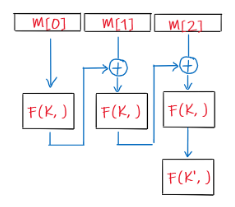
\includegraphics{cmac_construction.png}

	
	\subsection{Signature Scheme}
	A signature scheme has the same goals as a MAC, but avoids using a shared key by using a separate verification key and secret key. 
	\begin{itemize}[noitemsep, topsep=0pt]
		\item $\textsc{Gen}() \rightarrow (sk, vk)$ outputs two keys
		\item $\textsc{Sign}(sk, M) \rightarrow \sigma$ produces a tag for message $M$
		\item $\textsc{Ver}(vk, M, \sigma)$ that outputs 1 if $\sigma = \textsc{Sign(sk,M)}$.
	\end{itemize}
	
	\subsubsection{Security}
	Security definitions are the same as MAC, essentially. Gold standard is Existential Unforgeability under Chosen Message Attack.

	\subsubsection{Construction}
	The construction presented in class first built one-time security (each key pair can be used only once) for $n$-length messages by generating a random $sk$ matrix of size $2\times n$ where each entry is a bit, and a random $vk$ matrix that passes each bit of $sk$ through a one-way function. Then, the signature of the message is just selecting the top or bottom row depending on the value of each bit, and outputting the corresponding bit sequence. To verify, check that the one-way-function applied to each bit of the signature matches the output of the one-way-function applied to that bit that is stored in the verification key (corresponding to the given bit of the message). 

	This is then expanded to unbounded-length messages by hashing it first. \textbf{Hash then Sign} is also beneficial because it improves efficiency (signing a shorter message) and enhances security by effectively making the input to the function random (if we think of the hash function as a random oracle). We then only need random message attack security. 

	This is finally expanded to support many-time security by generating a new $sk, vk$ pair as above---one for every possible message. Then, even more secret keys are used to sign each pair of leaf verification keys, and produce a new verification key. This is repeated until eventually there remains just one verification key at the root: this is shared. To verify, the whole path must be verified to recompute the verificaiton key. Instead of precomputing these, which would be impossible, we generate them on the fly using a PRF. 
	
	\subsubsection{Practical Tools}
	Today, ECDSA-256 is most commonly used due to efficiency. However, SPHINCS-128 is secure against quantum computers.

	\vspace{2mm}
	\noindent\begin{tabular}{lcccc}
		Algorithm & PK Sz & Sig. Sz & signs/sec & ver/sec \\
		\hline
		SPHINCS-128 & 32B & 8000B & 5 & 750 \\
		RSA-2048 & 256B & 256B & 2000 & 50000 \\
		ECDSA-256 & 32B & 64B & 42000 & 14000 \\
		\hline
	\end{tabular}

	\subsection{Symmetric Encryption}

	\subsection{Security}
	\textbf{Indistinguishable under Chosen Plaintext Attack} (CPA Security) allows the attacker to send any number of pairs of encrypted messages. The challenger will then pick one and encrypt it according to its secret key, and return the ciphertext. The scheme is secure if the adversary can guess which of the two messages was encrypted with probability at most $\frac{1}{2} + \text{negl.}.$

	\textbf{\ldots Chosen Ciphertext Attacks} (CCA Security) is stronger, and allows the attacker to ask to see decryptions of ciphertext of messages of its choice in addition. The goal is the same as above. 

	\subsubsection{Construction}
	The construction given in class first uses a one-time pad of the length of the message. The ciphertext is then computed by XORing each bit of the message with the corresponding bit of the one-time pad. OTP is effectively randomizing the message to any outsider, so is secure against any computationally bounded attacker. But if any two ciphertexts are seen with the same pad, the XOR of the messages can be recovered: $c_1 = m_1 \oplus r, c_2 = m_2 \oplus r$, then $c_1 \oplus c_2 = m_1 \oplus m_2$. To fix this, a PRF is used to generate these pads from a short shared key. Using a PRF like AES allows only generating 128-bit pads, so we need a way of combining multiple. To do this, we can just add a counter and XOR the input to the PRF with this counter for each block. Now each block has a deterministic pad, and we can just output the concatenation of applying each pad to each block. This is CPA secure.

	But integrity is important for effective encryption, so it adds a MAC as well. To do this, it uses a separate key $k'$ for the MAC, and applies the MAC to the ciphertext, rather than to the plaintext then encrypting both together. This is to avoid any weird behavior caused by decrypting and acting on the message before verifying integrity, I think.

	\subsection{Diffie Hellman}
	Diffie-Hellman is a way of agreeing on a shared secret via a public communication channel.
	\begin{itemize}[noitemsep, topsep=0pt]
		\item publically agree on a large (2048 bits) prime $p$ and $g \in \{1\ldots p\}$, a generator modulo $p$.
		\item Alice chooses a random $a$ from $\{1\ldots p\}$, computes $g^a \mod p$, and sends it to Bob.
		\item Bob chooses random $b$ from $\{1\ldots p\}$ and sends $g^b \mod p$ to Alice.
		\item Each can then compute $g^{ab}$ by exponentiating the received value. This value is the shared secret.
	\end{itemize}

	The exponentiation can be done by repeated squaring, limiting multiplications required to $O(\log p)$. 

	\subsubsection{Security}
	Security relies on the \textit{Computational Diffie Hellman (CDH) Assumption}, which essentially says that $g^{ab}$ is hard to predict given $g, g^a \mod p, g^b \mod p$. This relies on the Discrete Log problem, or that $f(g) = g^x \mod p$ is one-way. Importantly, the key \textit{does not look random}---it is only unpredictable. The Decisional Diffie Hellman assumption allows stronger security by saying that $g^{ab}$ looks random, but it is false. This is because we can easily compute if something is a square. If we make $g$ be a square already, so that all values are squares, we can avoid this. In this case, and if $p=2q+1$ for some other prime $q$, it is believed that DDH is true, and that Diffie-Hellman is strongly secure. 

	\subsection{Public-Key Encryption}
	Allows encryption without a shared secret key. Implements three randomized algorithms that work on a message space:
	\begin{itemize}[noitemsep, topsep=0pt]
		\item $\textsc{Gen}() \rightarrow (sk, pk)$ outputs two keys
		\item $\textsc{Enc}(pk, m) \rightarrow ct$ produces a ciphertext for the message $m$
		\item $\textsc{Dec}(sk, ct) \rightarrow m$ outputs a message or fails
	\end{itemize}

	The goal is that a message encrypted with a certain user's public key can be decrypted only by that user's secret key, i.e. $\text{Pr}[\textsc{Dec}(sk, \textsc{Enc}(pk, m)) = m] = 1$.

	\subsubsection{Security}
	We have the same goals as in symmetric security. But CPA can be defined in a much simpler way, by stating that $(pk, \textsc{Enc}(pk, m)) \cong (pk, \textsc{Enc}(pk, m'))$, or that the encryption of any two distinct messages looks indistinguishable. We no longer have to explicitly allow the attacker to encrypt messages, because it has $pk$ and can thus do it on its own.

	However, the CCA definition looks the same as for symmetric encryption because the attacker cannot decrypt messages on its own.

	\subsubsection{Construction}
	The construction presented in class essentially just combines Diffie-Hellman with Symmetric Encryption, along with a hash function modeled as a random oracle to make the keys look random. To do this:
	\begin{itemize}[noitemsep, topsep=0pt]
		\item $\textsc{Gen}$ outputs $sk = a$ and $pk = g^a$
		\item \textsc{Enc} chooses a random $b$ and computes a key $K=H(pk^b)$ for the symmetric encryption. It then calls the symmetric encryption and outputs $(g^b, E(K, m))$, where $E$ is the underlying symmetric encryption method.
		\item \textsc{Dec}$(sk, (b, c))$ recomputes the shared key $K = H(b^{sk=g^a})$ and outputs $m=D(K,c)$, where $D$ is the symmetric decryption method.
	\end{itemize}


\section{Concepts}
\subsection{Delegation}
Many systems have several servers that each do something different, e.g. front-end server, processing server, DB. Each passes a request to the next, and it would be nice if those requests could be attached to the actual user request that caused it (so that a compromised server can't just do whatever it wants). Implicit delegation allows a server to just speak for all users: the server's identity is authenticated by the DB, for example, but not the users' identities. 

Explicit delegation is another design in which each server requires proof that the user asked the previous server to do something. This is usualy done by the user generating some cookie that has to do with their request, and then passing the cookie along through all the servers. Later servers can then verify that the user asked for the data. This can protect against malicious middle servers, but requires complex permission policies. 

% software security topics---not sure how to organize
\subsection{Privilege Separation}
Privelege separation is the idea that systems should be designed to minimize the damage of a compromise. This is done by breaking a system into components, and giving each component only the minimum privileges it needs to do its job. 

This provides a lot of benefits, because then a bug in one non-critical section of the code cannot delete the whole database or charge a million dollars to a credit card. But it also presents difficulties, because then there needs to be communication between the different components that must be secured. 

\subsection{Bug-Finding and Verification}
Many security problems are caused by bugs. Finding bugs is difficult, so there are many methods to try to find them. 

\subsubsection{Manual Testing}
Manual testing is basically just having some examples of what your code is expected to do and verifying that they do those things. It can capture corner cases and ensures that the code behaves correctly. However, the person writing the tests will probably forget about some corner cases, and in any case they cannot write tests for every possible case.

\subsubsection{Fuzzing}
Fuzzing is essentially a way of automating testing. It no longer checks correctness typically, but rather can be used to make sure that code does not crash for any input---the usefulness of this can be augmented by adding instrumentation to detect buffer overflows, etc and crash when they occur. 

The basic goal and benefit is to increase the coverage of the test cases. To do this, fuzzing programs usually start with a random input and continually modify it bit by bit. To achieve good test coverage, a metric that indicates how much of the code has been covered can be used to decide whether to keep a certain modification or not. Widely used. 

\subsubsection{Symbolic Execution}
Symbolic Execution is another way of finding crashes in a program. The basic idea is to pretend to run the program, but to do so where inputs are generic. Then, we can see whether crashes can be caused for any input rather than having to check individual inputs. 

To handle control flow, typically a SAT solver is used to see whether the condition for a jump is satisfied. Then the program can split to evaluate both cases. The set of constraints for each branch becomes more specific as this goes on, and they are stored. We can also use the SAT solver to find a satisfying assignment for each assertion that causes a crash, easily finding cases that the code does not handle. 

This works for simple examples, but becomes difficult with complex programs. 

\subsubsection{Formal Verification}
Formal Verification is a much stronger method of bug-finding that does actually prove correctness, since it verifies adherence to a strict spec. Proving correctness will eliminate many kinds of bugs. 


\subsubsection{Runtime Defenses}
Runtime defenses are a last-resort method of trying to achieve software security. They are measures that can be added to code execution to help prevent bugs from being so serious. 

\subsubsection{Stack Canary}
Basically just some magic number that is inserted between the function variables and the return address. If a buffer overflows towards the {\tt ra}, this will be overwritted before {\tt ra} is. Before returning, checks that this data is unmodified. Not perfect, since if an attacker knew the value used for the canary they could still overwrite {\tt ra}, but using a random value makes this unlikely.

\subsubsection{Address Space Layout Randomization}
Just randomly pick where process memory will go, so that adversary does not know where to jump. Makes the adversary's job a lot harder. 

\subsubsection{Fat Pointers}
Fat pointers are an idea to help limit the severity of buffer overflow bugs. Basically, each pointer now has a base and bound stored along with it. Anytime the pointer is dereferenced, the base and bound are checked to make sure that the pointer has not been corrupted.

This catches many issues, but not all---it does not protect against a buffer overflow overwriting within the same data structure as the buffer, which could allow overwriting the base and bound of a pointer and getting around the whole thing. It also does not protect against use-after-free bugs, which could allow a pointer to exist after something else is placed at the corresponding location. Also has a bit of overhead and changes the size of a pointer, which can be problematic. 

\subsubsection{Control Flow Ingegrity}
CFI builds a graph of all possible locations for computed jumps in code, and verifies that every jump is going somewhere that it is expected to go. This is not necessary for direct jumps, since they are guaranteed to be valid. Works pretty well, but still allows jumping to an incorrect location for the inputs, but still valid.

This will catch function pointer overwrites and stack canary bypass.

\subsubsection{Taint Tracking}
Taint tracking is essentially a method of tracking \textit{tainted} input data. This can be done by storing an extra bit along with every piece of input data, such as a string. There are \textit{sanitizing} operations that clear this bit, but most operations will leave it set. Then, when we pass the string to a SQL engine or something, we can halt the program if the string is still tainted/unsanitized. 

\subsection{Platform Trust}
\subsubsection{Secure Boot}
Secure boot is a method of establishing platform trust: trusting the underlying software and hardware stack. Essentially, its goal is to verify the software that is loaded on the computer. 

It does this in essence by storing a public key in ROM, that is hardwired when the computer is manufactured. When booting an operating system, it will check the signature of the operating system, and verify that the signature matches the hardcoded public key. If not, it will halt the boot. In technical implementation, needs to use a Merkle tree to verify since the whole OS cannot be loaded and hashed to verify at boot time---when loading later, the integrity of specific chunks can be checked against the tree.

\subsubsection{Measured Boot} 
Secure boot limits the software that can be run, which may not be desired. An alternative is Measured Boot, which provides different keys to different software, so if one OS encrypts the disk, a malicious OS cannot read back the disk data. This requires the hardware to have some durable secret inside it. The hardware can then derive a new key per-OS, based on the hash of the OS data. The OS then uses this key to derive new keys that it can do whatever it wants with. 

\subsection{Privacy with Leakage}
\subsubsection{Functional Encryption}
Encryption can completely hide a message, but sometimes this is too restrictive. For example, if all emails are encrypted, spam filters cannot work since the email server cannot see the email contents. We want to use a special encryption scheme that allows us to generate a new $sk$ \textit{for} a function $F$ that allows computing $F(m)$ from $\textsc{Enc}(sk, M)$ but does not allow learning anything else about $M$. There is a construction for leaking a single functional key but doing it with multiple keys seems much harder, nothing yet.

\subsubsection{Obfuscation}
The goal of obfuscation is to have a program that leaks nothing except the input/output of the program---no implementation details. Apparently, this can be used to construct pretty much every other cryptographic primitive. There is a way to have \textit{indistinguishable obfuscation}, where two programs with identical input/output behavior can be obfuscated to be indistinguishable. This is very inefficient, but it is polynomial.

\subsubsection{Zero-Knowledge Proofs}
The goal of zero-knowledge proofs is to prove you have some information without revealing the information itself. The current way of doing these uses interactive proofs. Basically, we ask the person a yes/no question that they would only know the answer to if they had the information. Then, there needs to be some way of checking if their response is valid. If it isn't, they are certainly lying, and if it is correct, the person may still be lying (they had a 50\% chance of guessing correctly). Repeat this until acceptable confidence is achieved. 

\subsection{Differential Privacy}
The goal of differential privacy is to allow performing operations on a dataset without revealing any information about any individuals in the dataset. This is only really achievable when there is some entity handling requests to the dataset---if we provide the whole dataset, we need to modify it so much that data is not useful. 

There must be a sanitizer that produces outputs based on the real dataset. The goal of this sanitizer is to provide outputs such that the true dataset cannot be distinguished with one where any single row is changed. This is done by adding noise. 
In order to determine how much noise must be added, we use the \textit{global sensitivity}. Global Sensitivity is essentially how much the function can change when a single row of the database changes:

\[ S(f) = \max_{\text{dist}(D, D') = 1} = |f(D) - f(D')| \]

In the above formula, $\text{dist}(D, D')$ is the number of differing rows between the two datasets. So if $f$ is the mean and the dataset values range from $a$ to $b$, the sensitivity is $\frac{b-a}{n}$. Once the global sensitivity is calculated, the output should be $f(D) + Z$, where $Z$ is the noise determined by:

\[ Z \sim \frac{S(f)}{\epsilon} \text{Lap}(0,1) \]

Where $\text{Lap}$ is the Laplace distribution.

\section{Systems \& Techniques}
\subsection{TLS}
TLS provides an \textit{encrypted and authenticated pipe} through which data can be transmitted between a client and a server. 

\subsubsection{Functionality}
It consists of two phases:
\begin{enumerate}[noitemsep, topsep=0pt]
	\item Handshake Phase: essentially diffie-helman key exchange between client and server, which is done in the clear. Once a shared key is established, communication is encrypted using the key. The server sends its certificate and signs the DH messages using the SK corresponding to this cert, so that the validity of the key exchange can be connected to the certificate.
	\item Record Protocol: once the client verifies that the certificate and exchanged messages are verified, the client and server communicate using the established shared key.
\end{enumerate}

\subsubsection{Properties}
TLS primarily provides correctness, prevents an attacker from learning the shared secret, and authentication of the server's identidy using certificate. Because new keys are generated for each session and deleted after, it also ensures that future compromise of the server does not leak past communication. Finally, it ensures that an adversary cannot impersonate the server unless the server's key is compromised. 

However, TLS \textit{does not} prevent an attacker from terminating the TLS connection, and does not hide the length of the ciphertext. 

This lack of length hiding had an interesting side effect with the CRIME attacks, where the request + response was gzipped then encrypted: by injecting a string into the request and observing the size change, one could see if that string was in the response without decrypting. 

\subsection{Mixnet}
A mixnet is a strategy to attempt to achieve metadata-private messaging: messaging that does not reveal the sender nor the receiver (nor sizes, timings, etc). Metadata-private messaging is achievable with \textit{rounds} if every client sends a message of the same size every round, regardless of whether they have something to send. However, this is not feasible, and breaks down when the attacker controls clients or the server. 

\subsubsection{Functionality}
In a mixnet, there is a chain of servers, each with $(pk_i, sk_i)$. Every client still must send a message every round. When a client wants to send a message, they encrypt $(\text{msg}, pk_{\text{dest}})$ first with the key of the last server, then with the key of the second-to-last server, etc. Finally, they send it to the first server in the chain. Each server shuffles the messages it received and strips off a layer of encryption, then sends to the next server in the chain. This continues until the last server receives the message and the destination public key. The last server then sends the message to its destination.

\subsubsection{Properties}
If a passive attacker does not control a certain server, it cannot tell which output messages correspond to which input messages. Therefore, a passive attacker can control \textit{all but one} of these servers, and still cannot tell who is sending what to who. 

However, it leaks who receives messages, and does not hold up well to active attackers, who can drop packets and do anything else.

\subsection{Fuzzy Extractor}
A fuzzy extractor can be used to derive a key from a noisy data source, such as a biometric or a Physically Uncloneable Function (PUF). Given a noisy $m$-length input bitstring $e$, the goal is to output an $n$-length derived key $s$, even when $e$ varies. The general strategy is to generate some public helper data $b$ of length $m$ that leaks information about $e$ and $s$ computed as follows, where $a_i$ are random and public $m$-length bitstrings.

\[
	\begin{aligned}
		b_1 & = a_1 \cdot s + e_1 \\
		b_2 & = a_2 \cdot s + e_2 \\
				& \ldots
	\end{aligned}
\]

Then, for a new noisy input $e'$, use $b$ and $a$ to reconstruct $s$ by solving the system of equations for $s$ using Gaussian elimiation. Importantly, only $n$ out of the $m$ total values are required to reconstruct $s$ (since it is of length $n$). Therefore, we can use confidence information provided by the biometric or PUF to only use the most confident $n$ values from $e'$. This allows us to essentially eliminate the noise.

\section{Labs}
\subsection{Lab 1}
Lab 1 focused on avoiding the attack where the server responds with a different photo than the client requested. To do this, we added an authenticated log to the server that . The server is untrusted, but we link the photo ID to a hash of the photo in the log, and store a MAC with a local secret alongside. When we download photos from the server, we verify that each log entry's MAC is valid and matches the downloaded photo blob.

\subsection{Lab 2}
Lab 2 implemented public-key infrastructure that was based on a chain of trust. So if Alice trusts Bob and Bob trusts Cedric, Alice has a trusted source for Cedric's public key through Bob. The way this works is that each person maintains a \textit{contact book} that stores the public keys of everyone they trust. Each of these is accompanied by a signature of that public key. Then, to get someone's public key through this chain, we can start by reading the next contact's public key from our own address book, and use this to verify signatures in their address book, and so on. 

\subsection{Lab 3}
Lab 3 implemented a private album feature that allowed adding and removing people from an album by their public key. To do this, we maintained a single shared key for each album. To share this key with friends, we essentially encrypted the shared key for their public key and posted it in the album metadata. To remove a friend, we changed the shared key and re-encrypted all photos. This also required that the album owner (the only one who can add/remove friends), signed the list of friends to ensure that no one added themselves.

\subsection{Lab 4}
Lab 4 interfaced with WebAssembly from Python to make edits to photos (the editing code was in WASM). To do this, we had to provide several methods in python-land that were then provided to the WASM code to use. These methods included things like opening photos, saving photos, and getting photo metadata. The main security consideration was that each instance of the WASM code is created with a \textit{tag} that grants it access to certain photos. We had to make sure that it could not read or modify photos that did not have that tag, and also should not be able to write photos that are marked read-only. To do this, the Python methods had to carefully check accesses. We also had to carefully check the inputs that the WASM code gave the python functions to ensure that the WASM code could not cause the Python code to crash.

\subsection{Lab 5}
Lab 5 was exploiting a dummy example of a timing side channel. We were given a verifier for secrets that verified them by iterating over the string and checking each letter, so the more correct letters, the longer it would take. To determine the secret, we then just had to guess one letter at a time, and time the verification to determine if the letter was correct or not---if the key with a certain letter took longer to verify, that letter should be correct. There was a lot of noise in this approach, though, so we needed to repeat the timing thousands of times for each letter. I implemented this by taking the letter that occurred most often over 100 trials, where each trial timed 10 verifications of each letter and took the one that took longest. This 100 trial limit is extended up to 5000 if there is no clear winner (won more than 20\% of trials). I also do a final verification, and start the whole process over if it fails, which it sometimes did. 

\end{multicols*}

\end{document}
